\documentclass[aspectratio=169]{beamer}

% Codage.  Ajuster en fonction de votre éditeur.  Supprimer avec LuaTeX.
\usepackage[utf8]{inputenc}

% Thème Beamer Télécom Paris.  Nombreuses options disponibles,
% cf. commentaires ci-dessous et slides de démonstration dans
% corps du document.
\mode<presentation>
\usetheme{tptng}

\setlength{\tptframetitleyshiftifsubtitle}{16pt}

% Les options s'utilisent via \usetheme ci-dessus, ou bien via \tptthemekeys.
% P.ex. \tptthemekeys{visual} est équivalent à \usetheme[visual]{tptnew}.
%
% Options simples :
%
% • official (défaut) copie fidèlement la charte graphique officielle.
% • visual rend la charte plus lisible, notamment le contraste des gris.
% • slim réduit l'encombrement du titre des frames.
% • nohelvet garde les polices par défaut.
% • latex garde les polices par défaut et les symboles de navigation Beamer.

% Vous pouvez aussi ajuster les marges en décommentant :
% \setbeamersize{text margin left=1cm, text margin right=1cm}

% Gestion des fontes.  Attention, le code à utiliser dépend du moteur TeX.
\iftptusefontspec
  % Utiliser ce code avec LuaTeX et XeLaTeX.
  \setmonofont{inconsolata}% Police monospace (p.ex. pour l'adresse mail).
\else
  % Utiliser ce code avec pdfTeX et le vieux TeX original.
  \usepackage[T1]{fontenc}
  %\usepackage{lmodern}% Recommandé si vous activez l'option latex ou nohelvet.
  \usepackage{inconsolata}% Police monospace (p.ex. pour l'adresse mail).
\fi

% Gestion des images.  Le thème a déjà chargé graphicx.  Pour préciser
% les dossiers où se trouvent les images, et ne pas avoir à spécifier
% leur extension dans les noms de fichiers :
\graphicspath{{images/}{pdfs/}{figs/}{svgs/}{odgs/}{bitmap/}}
\DeclareGraphicsExtensions{.fig,.pdf,.png,.jpg}

% Pour insérer directement des images au format .fig :
\usepackage{figlatex}

% Divers : typographie française, gestion des tables,
% programmation de dessins, calcul de longueurs, date, texte de remplissage.
% Supprimez ce dont vous n'avez pas besoin.
\usepackage[french]{babel}
\usepackage[babel]{microtype}
\usepackage{booktabs}
\usepackage{tikz}
\usepackage{calc}
\usepackage[useregional]{datetime2}
\usepackage{siunitx}


%%------------------------------------------------------------------------------

% Faire apparaître le plan à chaque section et sous-section :
\AtBeginSection[]{
  \contentsframe[currentsection]
}
\AtBeginSubsection[]{
  \contentsframe[currentsection,currentsubsection]
}
% Avec un autre nom que «Table des matières» en français.
\renewcommand*{\contentsframename}{Plan}

%------------------------------------------------------------------------------


%------------------------------------------------------------------------------
\title[MAPRENE-XXI]{Modélisation d'amplificateur de puissance par réseaux de neurones}
\subtitle{Projet PAF}

\author{Germain Pham \& Chadi Jabbour}
\email{dpham@telecom-paris.fr}
\institute{C2S - Télécom Paris}
\date[2020-06-21]{\DTMdate{2020-06-21}}% Ou simplement \date{\today}.

% Logo additionnel sur la page de titre (pour une conf ou un évènement).
% \logotitleextra*[width=3.5cm]{logo-PAF-MAPRENE}
\logotitleaffiliation*[width=3.5cm]{logo-PAF-MAPRENE}
\setlength{\footerlogoheight}{2em}
\setlength{\footerlogoyshift}{0pt}
\logofootermain{%   Sans * : code brut.
  \hspace*{\footlinespacing}%
  \includegraphics[height=\footerlogoheight,page=2]{logo-PAF-MAPRENE}
  }

%------------------------------------------------------------------------------
\begin{document}

\maketitle

\section{Introduction}

\begin{frame}
  \frametitle{\insertsection}

      \begin{columns}
        \begin{column}{0.5\textwidth}
          \footnotesize
          \begin{itemize}
            \item Systèmes de télécommunication
          \end{itemize}
          \vspace{-\baselineskip}
          \begin{center}
            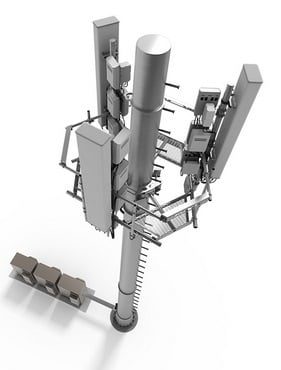
\includegraphics[width=0.6\textwidth]{medium}
          \end{center}
        \end{column}
        \begin{column}{0.7\textwidth}
          \begin{center}
            \includegraphics[width=\textwidth]{2021TutorialRFIC-Pham-Degreys-V2-notes-pruning-noteless-extract}\\
          \vspace{0.5\baselineskip}
          \includegraphics[width=0.5\textwidth]{2010-AnalyzingLINCSystems--IEEEJournals--Magazine--IEEEXplore-extract}
          \end{center}
        \end{column}
      \end{columns}

{\tiny \vspace{0.5\baselineskip}
  Sources: \href{https://manometcurrent.com/global-lte-base-station-antenna-market-2020-industry-scenario-strategies-growth-factors-and-forecast-2025/}
{Global LTE Base Station Antenna Market 2020} ; Birafane [2010] - Analyzing LINC Systems}

\end{frame}

\begin{frame}
  \frametitle{\insertsection}

  \footnotesize
  \vspace{-0.5\baselineskip}
  \begin{columns}[t]
    \begin{column}{0.45\textwidth}
      \begin{itemize}
        \item Apprentissage artificiel
      \end{itemize}
      \vspace{-0.5\baselineskip}
      \begin{center}
        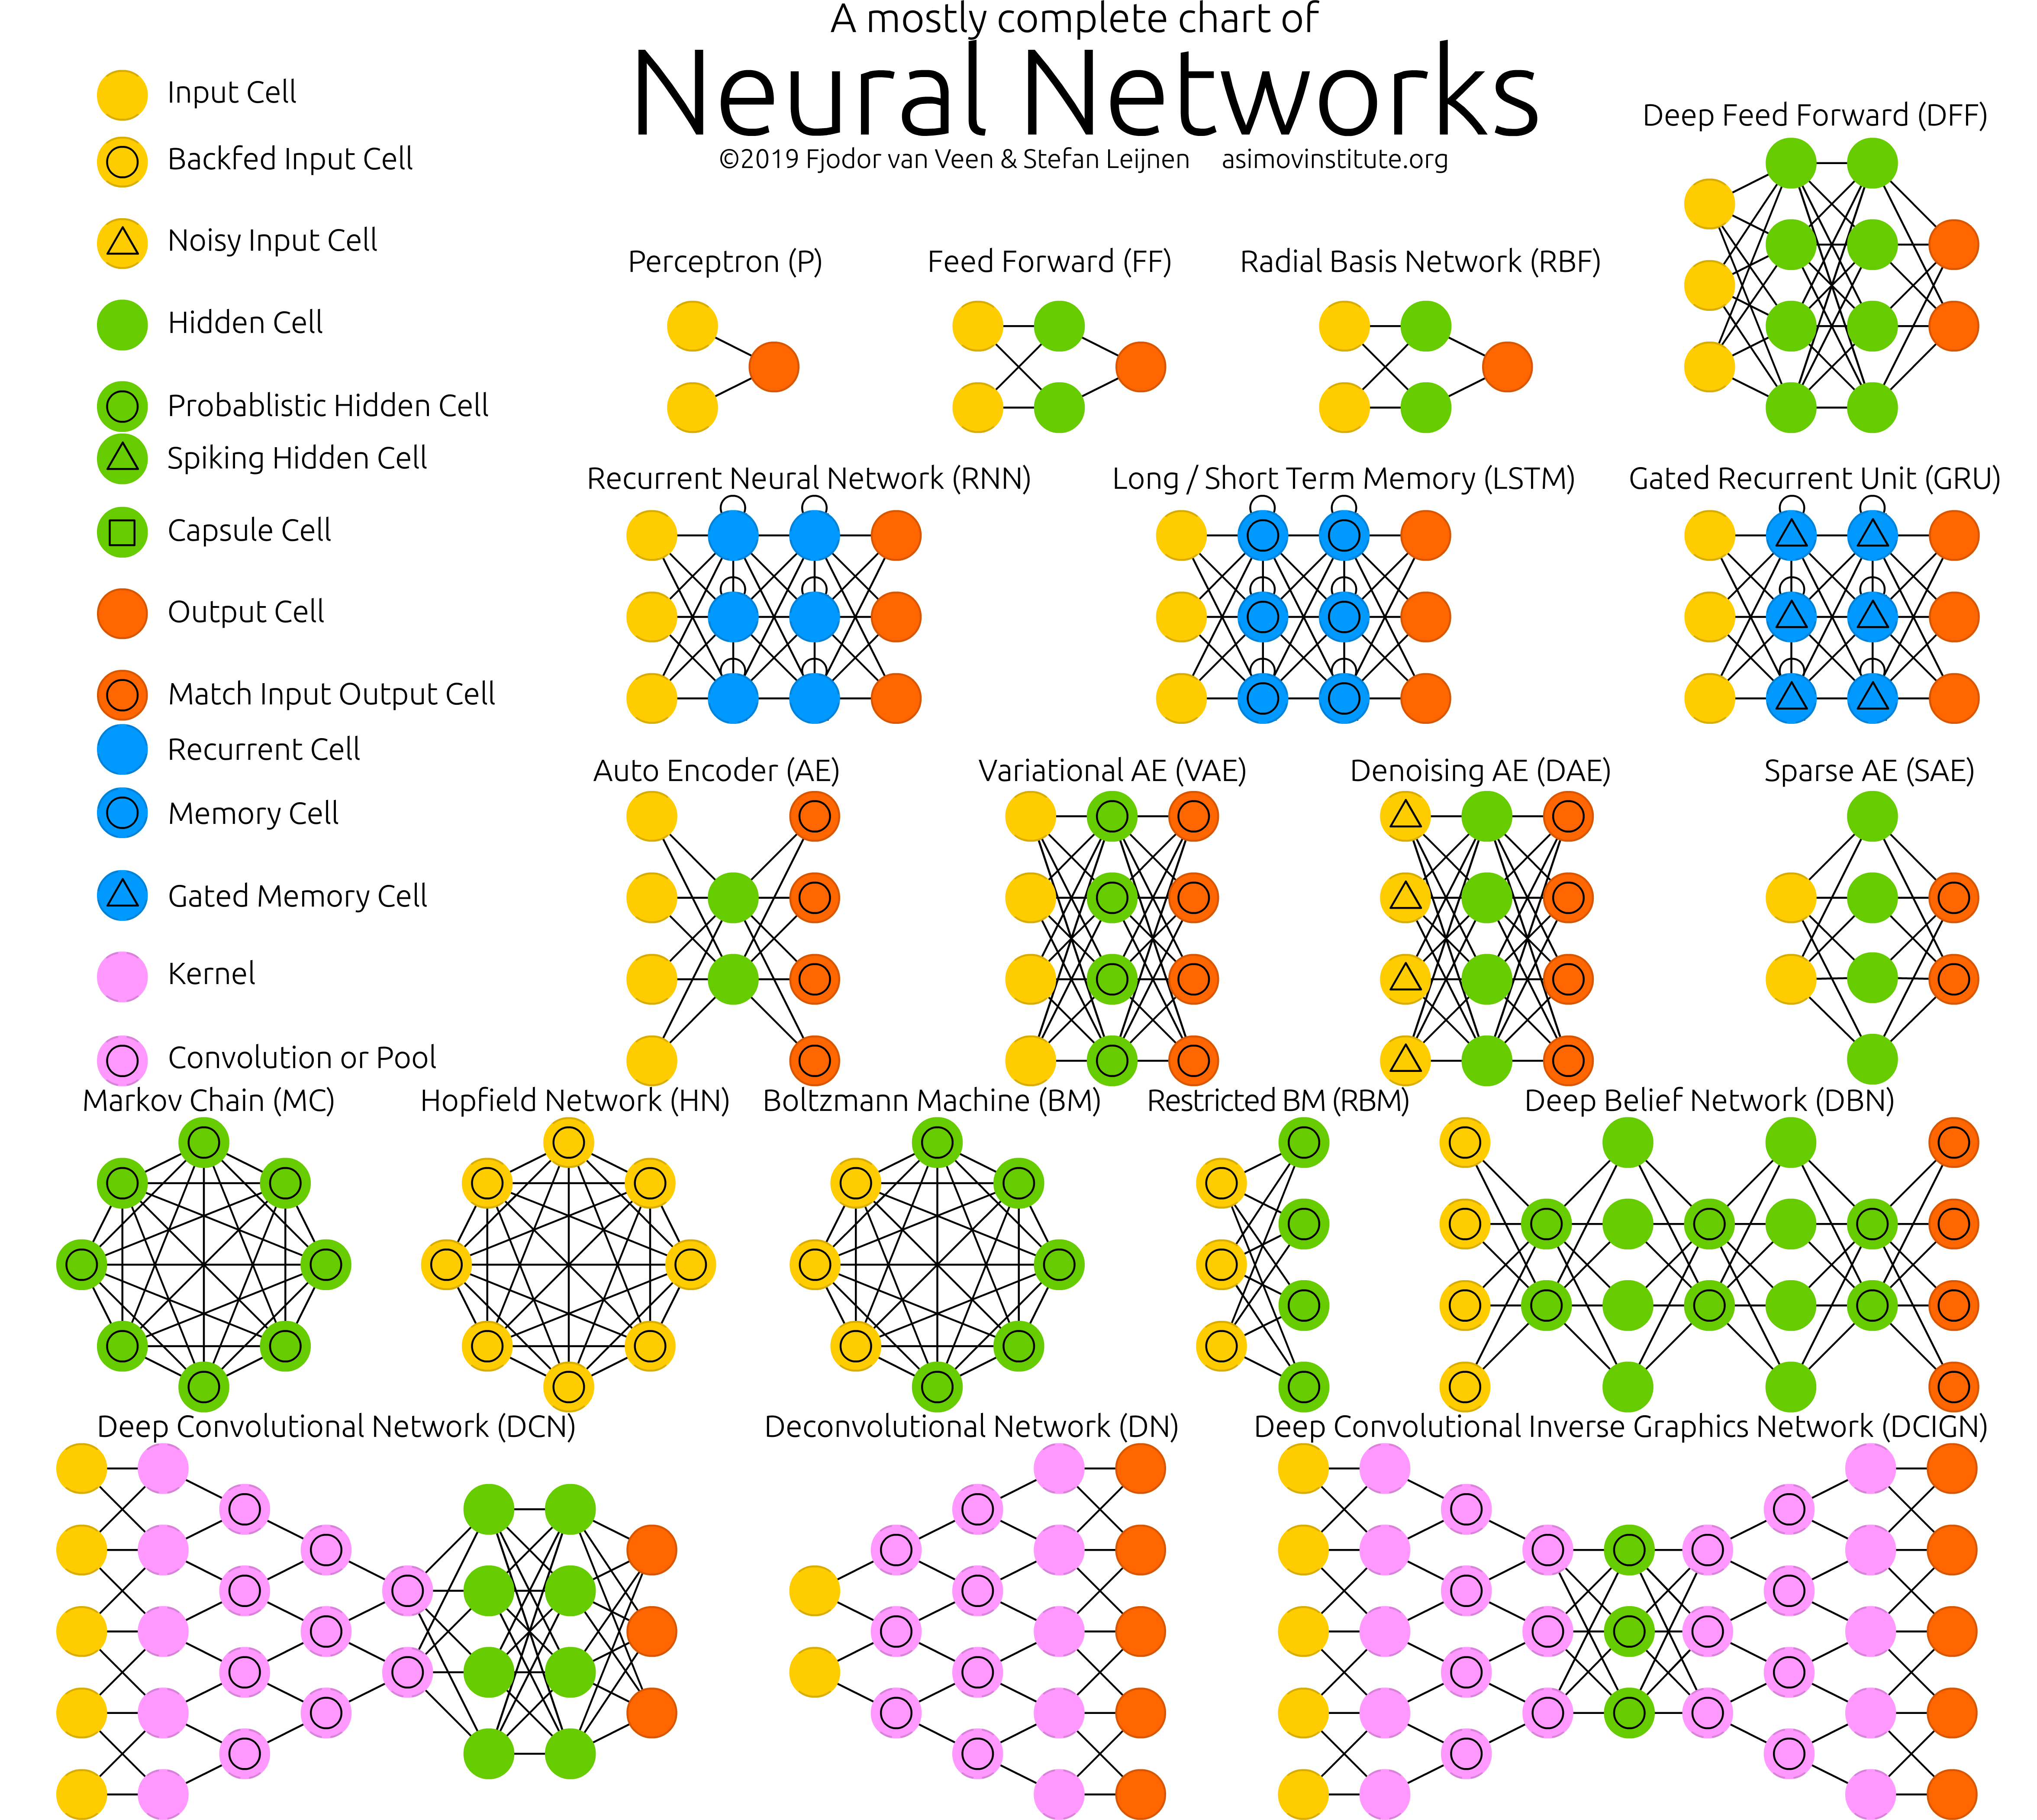
\includegraphics[width=\textwidth]{NeuralNetworkZo19High-lite}
      \end{center}
    \end{column}
    \begin{column}{0.65\textwidth}
      \begin{block}{Théorème d'approximation universelle}
        Les réseaux de neurones peuvent approximer n'importe quelle fonction continue
      \end{block}
      \vspace{-\baselineskip}
      \begin{center}
        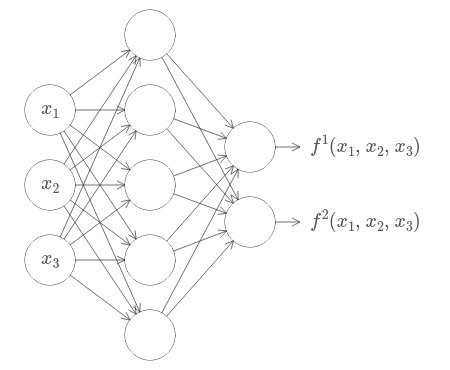
\includegraphics[width=0.45\textwidth]{vector-valued-network}
      \end{center}
      \vspace{-\baselineskip}
      Plus d'infos : \href{https://ai.stackexchange.com/questions/13317/where-can-i-find-the-proof-of-the-universal-approximation-theorem/13319}
      {Where can I find the proof of the universal approximation theorem?}
    \end{column}
  \end{columns}

  {\tiny \vspace{0.5\baselineskip}
  Sources : \href{https://www.asimovinstitute.org/neural-network-zoo/}
  {The Neural Network Zoo - The Asimov Institute ; 
  \href{http://neuralnetworksanddeeplearning.com/chap4.html}
  {A visual proof that neural nets can compute any function}
  }
  }
\end{frame}

\section{Bases théoriques}

\begin{frame}
  \frametitle{\insertsection : Modélisation d'amplificateur}
  \vspace{-0.5\baselineskip}
  \begin{columns}[T]
    \begin{column}{0.5\textwidth}
      \begin{itemize}
        \item Amplificateur de puissance
      \end{itemize}
      \includegraphics[width=0.49\textwidth]{2016-Ajointlinearity-efficiencymodelofradiofrequencypoweramplifiers--IEEEConferencePublication--IEEEXplore-extract}
      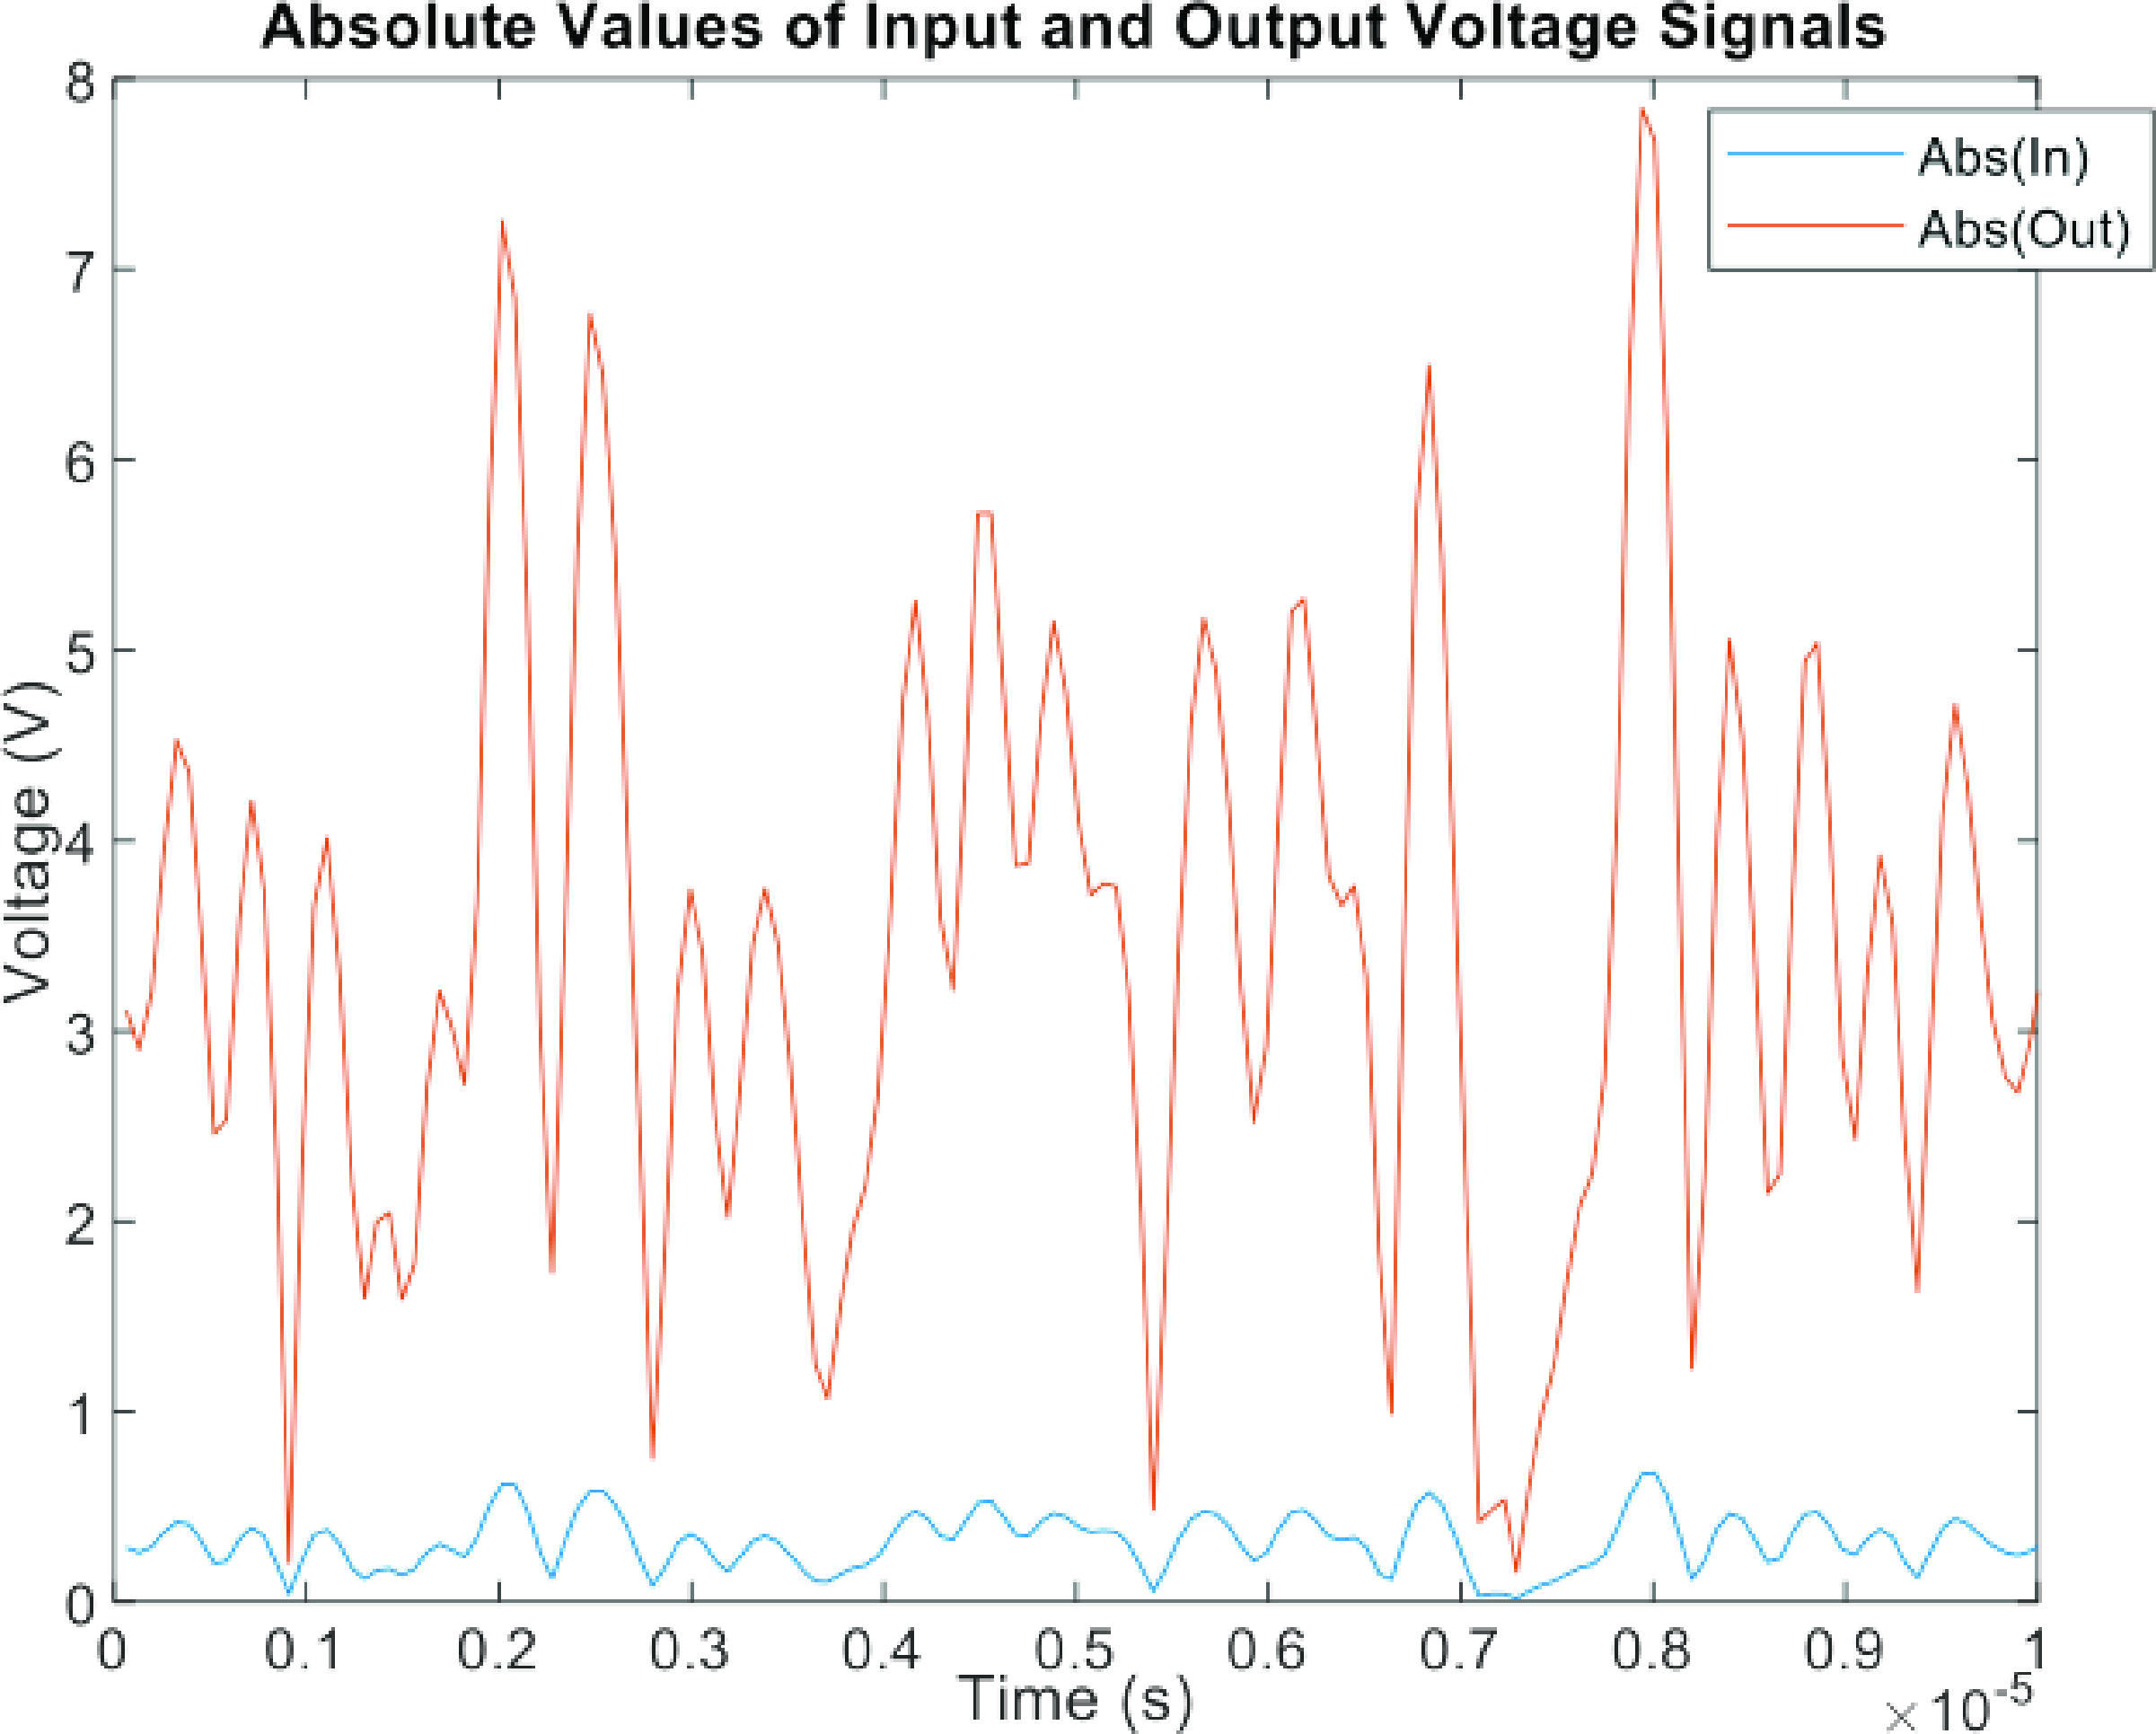
\includegraphics[width=0.49\textwidth]{modelling-rf-power-amplifiers-with-dpd-using-matlab-white-paper-extract-5}
      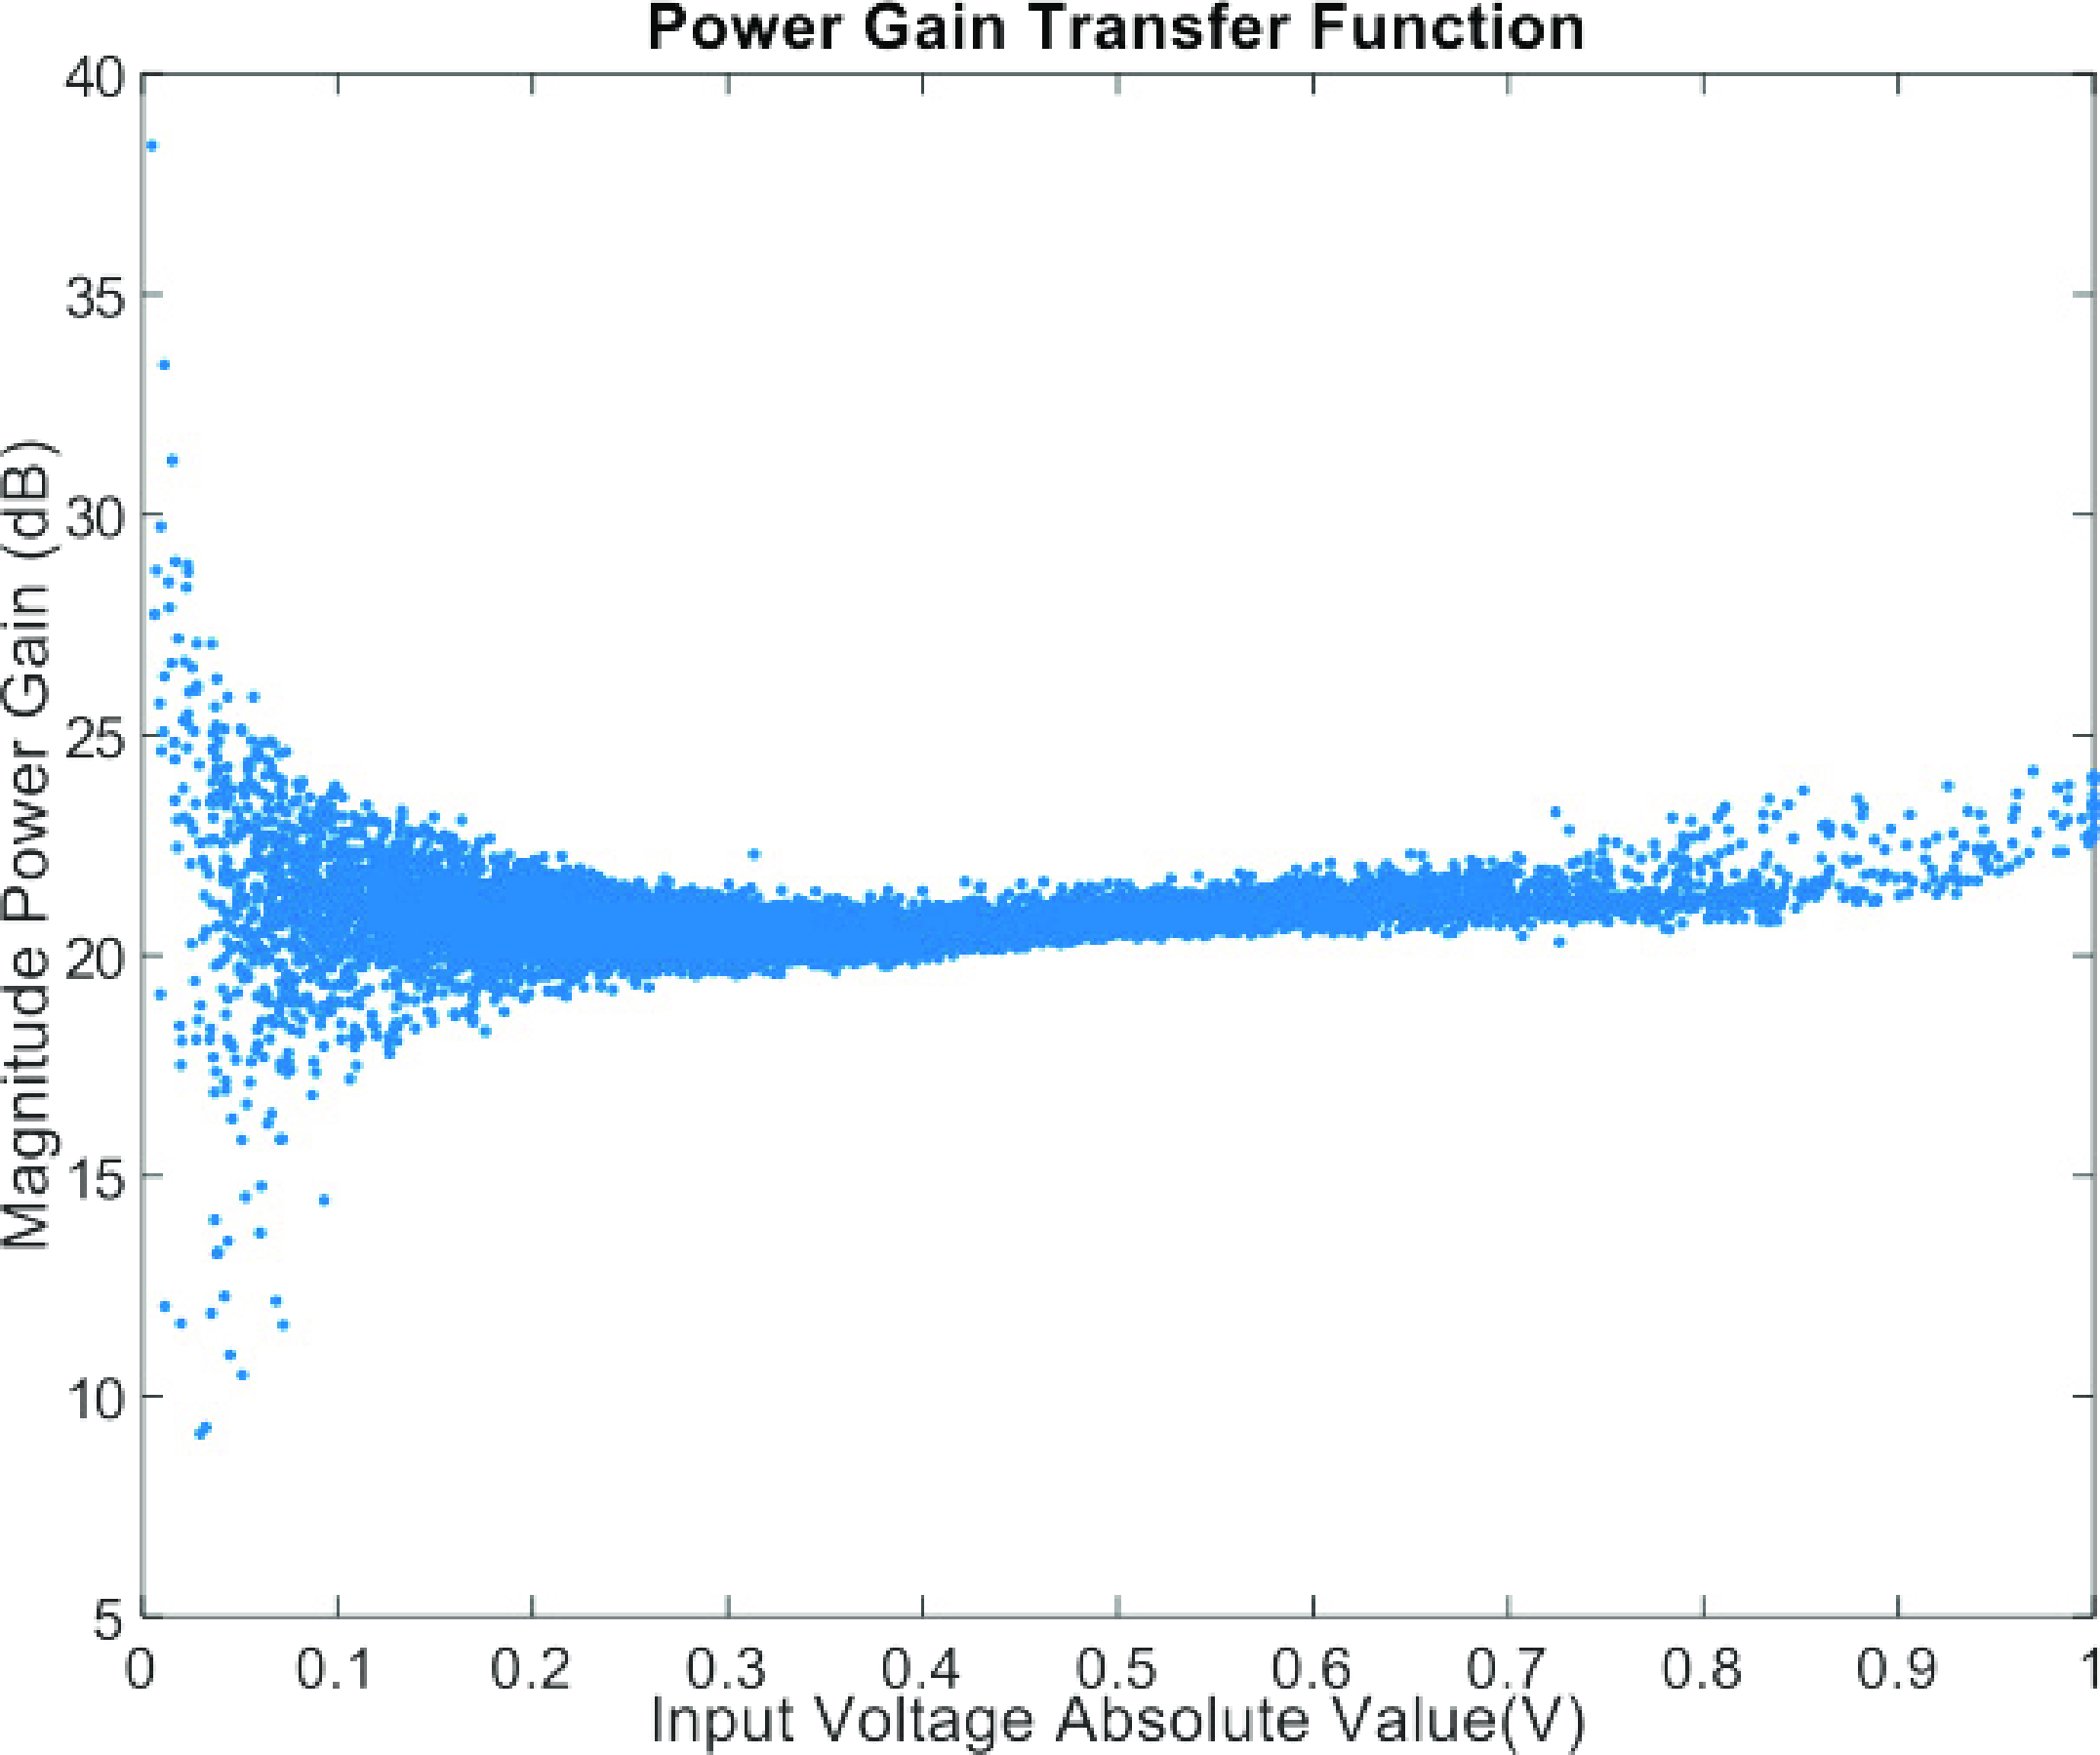
\includegraphics[width=0.49\textwidth]{modelling-rf-power-amplifiers-with-dpd-using-matlab-white-paper-extract-6}
      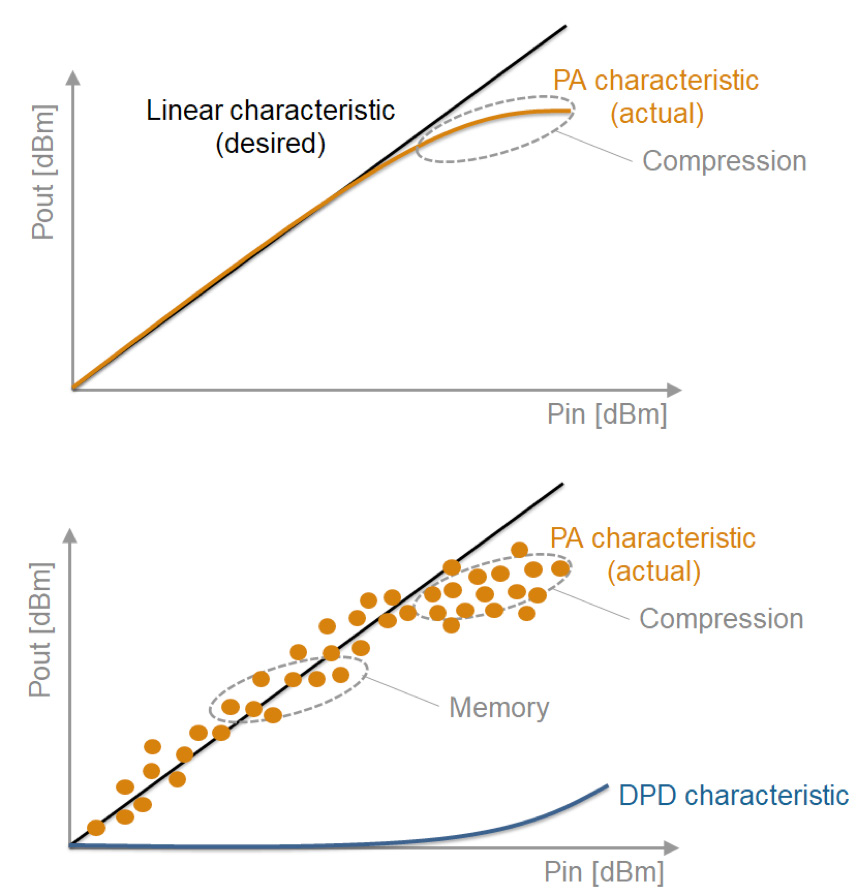
\includegraphics[width=0.49\textwidth]{modelling-rf-power-amplifiers-with-dpd-using-matlab-white-paper-extract-pic-002}
    \end{column}
    \begin{column}{0.6\textwidth}
      \begin{itemize}
        \item Illustration d'un "Fitting"
      \end{itemize}
      \vspace{-0.5\baselineskip}
      \begin{center}
        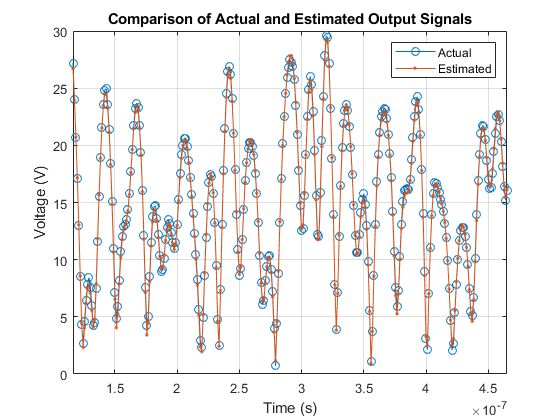
\includegraphics[width=0.49\textwidth]{PowerAmplifierCharacterizationExample-05}
        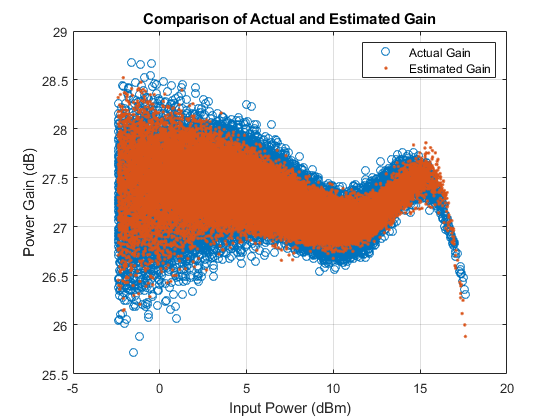
\includegraphics[width=0.49\textwidth]{PowerAmplifierCharacterizationExample-08}
      \end{center}
      \vspace{-\baselineskip}
      \begin{itemize}
        \item Exemples de fonctions non-linéaires
      \end{itemize}
      \vspace{-0.5\baselineskip}
      \begin{center}
        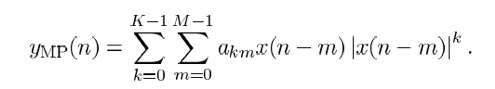
\includegraphics[width=0.49\textwidth]{modelling-rf-power-amplifiers-with-dpd-using-matlab-white-paper-extract-pic-008}\\
        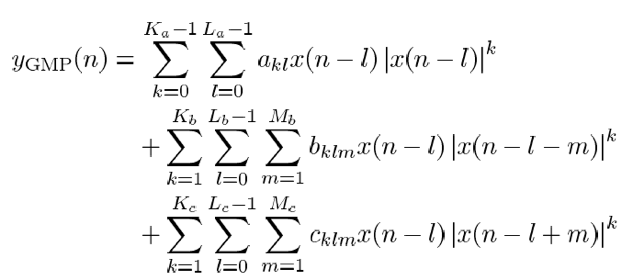
\includegraphics[width=0.49\textwidth]{modelling-rf-power-amplifiers-with-dpd-using-matlab-white-paper-extract-pic-010}
      \end{center}
    \end{column}
  \end{columns}

\end{frame}

\begin{frame}
  \frametitle{Modélisation et précision}
  \vspace{-\baselineskip}
  \begin{columns}
    \begin{column}{1.2\textwidth}
      \footnotesize
      \begin{itemize}
        \item Qu'est-ce qu'un bon modèle ?
        \begin{itemize}
          \footnotesize
           \item Un bon modèle permet de reproduire fidèlement le comportement d'un système. 
           Idéalement, la sortie d'un modèle doit être identique aux mesures.
           \item Sa complexité doit être prise en compte
        \end{itemize}
     \end{itemize}
    \end{column}
  \end{columns}
  \begin{columns}[t]
    \begin{column}{0.4\textwidth}
      \footnotesize
     \begin{itemize}
       \item Méthodologie
     \end{itemize}
       \begin{center}
        \includegraphics[width=0.8\columnwidth]{B_PAmodeling}\\
        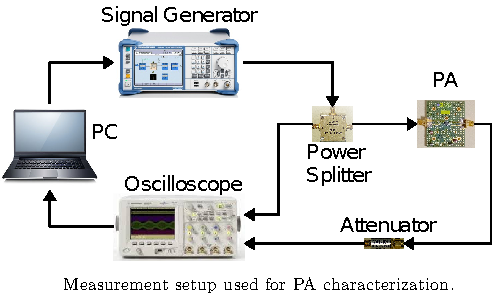
\includegraphics[width=0.8\columnwidth]{PAsetup}
       \end{center}
    \end{column}
    \begin{column}{0.6\textwidth}
      \footnotesize
     \begin{itemize}
       \item Évaluation de la performance (domaine temporel)
       \begin{itemize}
             \item Normalized Mean Square Error
       \end{itemize}
     \end{itemize}
     \begin{equation}
          NMSE = 10 \log_{10} \left ( \frac{ \sum_{\ell=1}^{L} \left | y_{model}(\ell) - y_{meas}(\ell) \right |^2 }{\sum_{\ell=1}^{L}  \left | y_{meas}(\ell) \right |^2 }  \right )
    \end{equation}
    \end{column}
    \begin{column}{0.05\textwidth}
      
    \end{column}
  \end{columns}



\end{frame}

\begin{frame}
  \frametitle{\insertsection : Apprentissage artificiel}
  
  \begin{columns}
    \begin{column}{0.7\textwidth}
      Thématique très vaste\\
      \footnotesize
      Ressources pour commencer : 
      \begin{itemize}
        \item Perceptron multi-couche : 
        \href{https://penseeartificielle.fr/focus-reseau-neurones-artificiels-perceptron-multicouche/}
        {Focus : Le Réseau de Neurones Artificiels ou Perceptron Multicouche}
        \item Diapos d'introduction RNN (français) : 
        \href{https://perso-etis.ensea.fr/luvizon/pluxml/Neurones.pdf}
        {Introduction aux réseaux de Neurones (ENSEA)}
        \item Les frameworks de ML : 
        \begin{itemize}
          \footnotesize
          \item scikit-learn : \url{https://scikit-learn.org/stable/}
          \item Tensor Flow : \url{https://www.tensorflow.org/resources/learn-ml?hl=fr}
        \end{itemize}
      \end{itemize}
    \end{column}
    \begin{column}{0.35\textwidth}
      \includegraphics[width=\columnwidth]{2020-RethinkingMotivationofDeepNeuralArchitectures--IEEEJournals--Magazine--IEEEXplore-extract}\\
      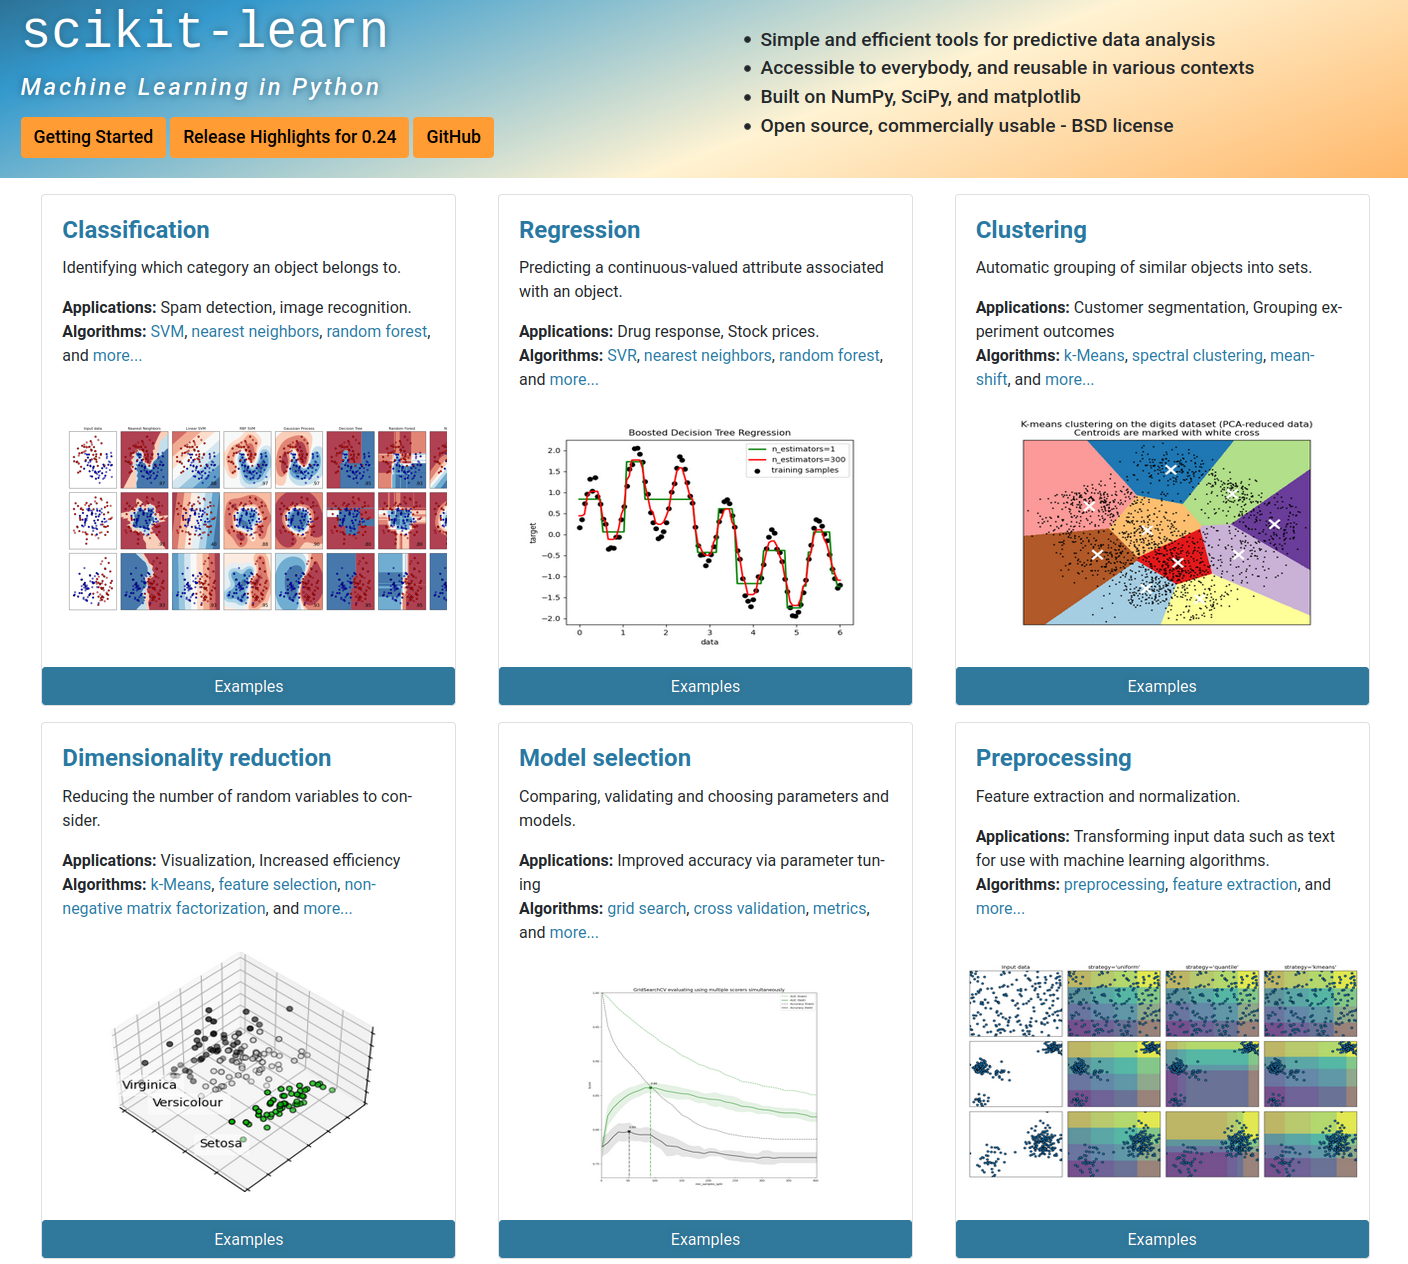
\includegraphics[width=\columnwidth]{scikit-learn}
    \end{column}
  \end{columns}

  {\tiny
  Source : 2020 - Rethinking Motivation of Deep Neural Architectures
  }
\end{frame}

\begin{frame}
  \frametitle{\insertsection : Apprentissage artificiel}

\begin{columns}
  \begin{column}{0.5\textwidth}
    Vos mots clés : 
    \begin{itemize}
      \item Perceptron multi-couche (multi layer perceptron)
      \begin{itemize}
        \item Fonction d'activation : sigmoïde
      \end{itemize}
      \item Rétropropagation de l'erreur (backpropagation)
    \end{itemize}
  \end{column}
  \begin{column}{0.6\textwidth}
    \begin{center}
      \includegraphics[width=\textwidth]{NeuralNets}
    \end{center}
  \end{column}
\end{columns}



  

\end{frame}


\section{Flot de travail}

\begin{frame}
  \frametitle{\insertsection}
\footnotesize
  \begin{columns}[t]
    \begin{column}{0.6\textwidth}
      Implémenter la modélisation PA avec NN
      \begin{itemize}
        \item Installer les librairies Python + ML (scikit learn/tensorflow)
        \item Comprendre les bases de NN
        \begin{itemize}
          \footnotesize
          \item Effectuer des exemples de classification simples
          \item Effectuer un exemple de fitting non linéaire
        \end{itemize}
        \item Implémenter un filtre non linéaire basé sur MLP
        \item Implémenter le BP pour entrainer un filtre NL basé sur MLP
        \item Rédiger de la documentation
      \end{itemize}
    \end{column}
    \begin{column}{0.6\textwidth}
      Effectuer des mesures PA et appliquer la modélisation
      \begin{itemize}
        \item Mesures
        \begin{itemize}
          \footnotesize
          \item Générer un stimulus (LTE) avec python (ou Matlab)
          \item Transférer le stimulus au générateur de signaux
          \item Configurer le matériel de sonorisation
          \item Exciter l'ampli avec le stimulus et acquérir les signaux RF
          \item Post-traiter les signaux mesures (RF vers bande de base, alignement, filtrage, sous-échantillonnage)
        \end{itemize}
        \item Appliquer la modélisation
        \item Rédiger de la documentation
      \end{itemize}

    \end{column}
  \end{columns}

\end{frame}

\section{Livrables}

\begin{frame}
  \frametitle{\insertsection}

  \begin{itemize}
    \item Courbes NMSE vs hyperparametres du réseau (nombres de neurones)
    \begin{itemize}
      \item Neurones d'entrée = mémoire : de 0 à 4 pour chaque voie (I et Q)
      \item Neurones cachés : de 50 à 200
      \item Neurones de sortie : 1 (somme complexe)
    \end{itemize}
    \item Codes Python sur Git
    \begin{itemize}
      \item Des messages de \texttt{commit} de qualité. 
      \item Un \texttt{push} tous les deux jours au moins. 
    \end{itemize}
    \item Documentation
    \item Un poster + une démo
  \end{itemize}

\end{frame}


\begin{frame}
  \frametitle{Encadrants et spécialités}
\small
  \begin{columns}
    \begin{column}{0.6\textwidth}
      \begin{itemize}
        \item Germain Pham (3B46)
        \begin{itemize}
          \item Traitement du signal
          \item Modélisation d'ampli
          \item Programmation Python
          \item Bases de machine learning
        \end{itemize}
      \end{itemize}
      \begin{itemize}
        \item[]\begin{itemize}
          \item Disponible : sauf mention contraire : tous les jours à partir de $\approx\SI{9}{h}$
          \item Indisponible : 
          \begin{itemize}
            \item les lundi et jeudi à partir de 17h30
            \item les mercredi après-midi (à partir de 13h30)
            \item ce vendredi 25 juin toute la journée
          \end{itemize}
        \end{itemize}
      \end{itemize}
    \end{column}
    \begin{column}{0.6\textwidth}
      \begin{itemize}
        \item Chadi Jabbour (3B44 ?)
        \begin{itemize}
          \item Traitement du signal
          \item Modélisation circuits télécom
          \item Mesures matérielles
        \end{itemize}
      \end{itemize}
      
    \end{column}
  \end{columns}

\end{frame}

\end{document}
